\documentclass[crop,tikz]{standalone}
\usetikzlibrary{backgrounds}
\colorlet{blue}{cyan}
\tikzset{
  inverted/.style = {
    color=white,
    background rectangle/.style={fill},
    show background rectangle
  }
}
\usepackage{pgfplots}
\pgfplotsset{compat=1.18}

% Flow around a circle.
%
% Derived by trasforming the uniform flow f(w) = w via the Joukowski
% mapping J(z) = (z + 1/z)/2. The resulting complex potential is given
% by g(z) = f(J(z)) = (z + 1/z)/2. Taking z = r e^{i\phi}, the flow
% lines are given by Im(g(z)) = 1/2(r - 1/r)sin(\phi) = constant = c.
% Solving this last equation for r(\phi) yields
% r(\phi) = c/sin(\phi) +- sqrt(1 + (c/sin(\phi))^2)

\pgfplotsset{
  inverted/.style = {
    every axis legend/.append style={
      draw=white,
      fill=black,
      text=white
    }
  },
}

\begin{document}
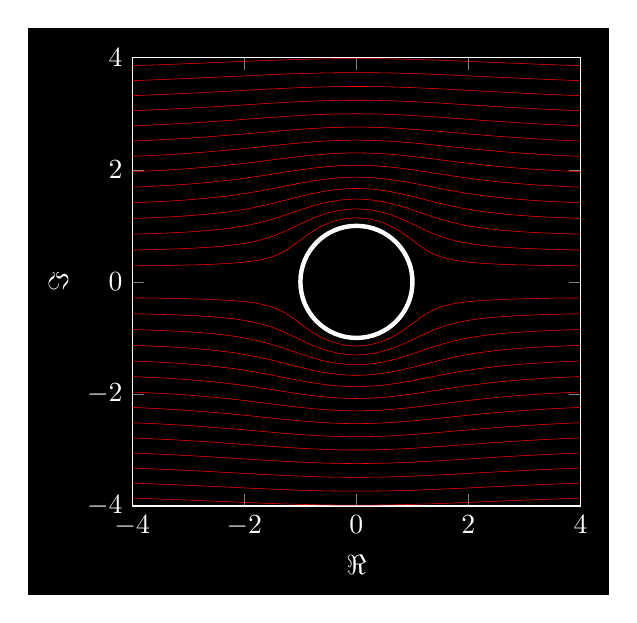
\begin{tikzpicture}[inverted,inverted]
  \pgfmathsetmacro{\numberoffieldlines}{30};
  \pgfmathsetmacro{\numberofpotentiallines}{15};
  \pgfmathsetmacro{\remin}{-4};
  \pgfmathsetmacro{\remax}{4};
  \pgfmathsetmacro{\immin}{-4};
  \pgfmathsetmacro{\immax}{4};
  \pgfmathsetmacro{\cmin}{0};
  \pgfmathsetmacro{\cmax}{4};
  \begin{axis}[inverted,
    axis equal image,
    xmin={\remin}, xmax={\remax},
    ymin={\immin}, ymax={\immax},
    xlabel={$\Re$},
    ylabel={$\Im$},
    samples=100,
    domain=3:177,
    declare function = {
      % flow lines
      fr(\x,\c,\s) = \c/sin(\x) + \s*sqrt(1 + (\c/sin(\x))^2); % radius r as a function of \phi, \s = sign
      fc(\n,\nmax) = \cmin + \n/\nmax*(\cmax - \cmin); % calculates c
      % lines of constant potential
      pr(\r,\c) = 2*\c*\r/(1 + \r^2); % cos(\phi) as a function of r
      pc(\n,\nmax) = -1 + 2*\n/\nmax; % calculates c
    },
    ]
    % flow lines
    \pgfplotsinvokeforeach{1,...,{\numberoffieldlines}}{
      \addplot[red,very thin] (
        {fr(x,fc(#1,\numberoffieldlines),1)*cos(x)},
        {fr(x,fc(#1,\numberoffieldlines),1)*sin(x)}
      );
      \addplot[red,very thin] (
        {fr(x,-fc(#1,\numberoffieldlines),-1)*cos(x)},
        {fr(x,-fc(#1,\numberoffieldlines),-1)*sin(x)}
      );
    }
    % lines of constant potential
    % \pgfplotsinvokeforeach{0,...,{\numberofpotentiallines}}{
    %   \addplot[blue,very thin,domain=1:{\remax+1}] (
    %     {x*pr(x,pc(#1,\numberofpotentiallines))},
    %     {x*sqrt(1 - pr(x,pc(#1,\numberofpotentiallines))^2)}
    %   );
    %   \addplot[blue,very thin,domain=1:{\remax+1}] (
    %     {x*pr(x,pc(#1,\numberofpotentiallines))},
    %     {-x*sqrt(1 - pr(x,pc(#1,\numberofpotentiallines))^2)}
    %   );
    % }
    % circle
    \draw[ultra thick] (0,0) circle (1);
  \end{axis}
\end{tikzpicture}
\end{document}
